% Licensed under the Creative Commons Attribution Share Alike 4.0 International.
% See the LICENSE file in the repository root for full license text.

\section{实验:CMake 的基本工作流程\label{sec:experiment-3}}

图 \ref{fig:cmake-gui-2} 中,需要在最上面的编辑框中填写源代码所在目录。CMake 程序并不直接帮助你搜集该目录下源代码的信息,而是根据目录下名为 \lstinline[language={}]{CMakeLists.txt} 的文本文件进行工作。所以,学习 CMake 实际上是指学习编写 \lstinline[language={}]{CMakeLists.txt} 文件,我们将从下一章开始讨论。本实验中,我们将聚焦 CMake 程序的使用方法。

\subsection*{实验步骤}

\begin{enumerate}
	\item 新建空白 CMakeLists 文件。在工作目录下新建文件夹,并在其中新建一个文本文件,命名为 \lstinline[language={}]{CMakeLists.txt}。

	\begin{note}
		没错,尽管其他教程可能已经开始教你如何建立一个最小工程了,但我们在两章后才做这件事。现在的 \lstinline[language={}]{CMakeLists.txt} 就是一个空文件。
	\end{note}

	\item 在 cmake-gui 中打开新建的文件夹。

	从开始菜单打开 cmake-gui,点击“Brouse Source...”按钮,选择刚才新建的文件夹。再将图 \ref{fig:cmake-gui-2} 中“生成文件的目录”设定为工作目录下的另一个文件夹(通常以 \lstinline[language={}]{build} 开头命名),如图 \ref{fig:empty-cmake-1} 所示。

	\begin{figure}
		\centering
		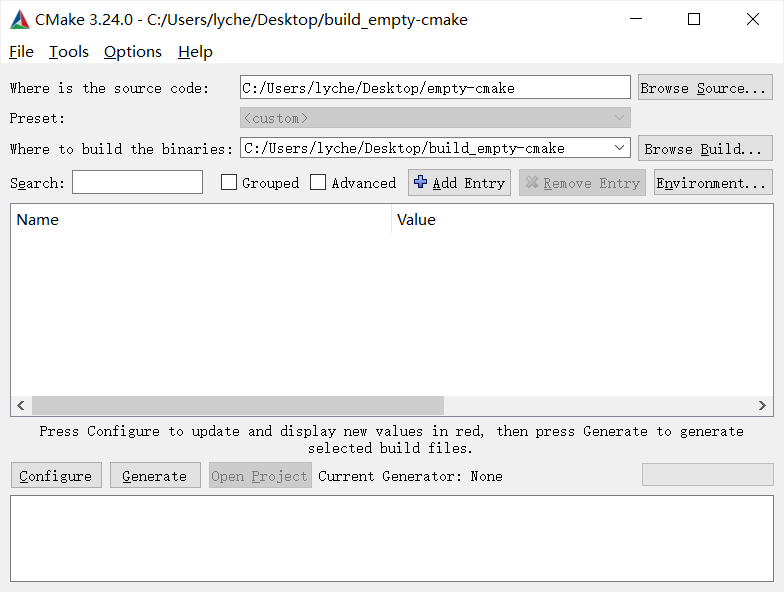
\includegraphics[width=0.75\linewidth]{assets/empty-cmake-1}
		\caption{填写源代码所在目录和生成文件目录的示例。}
		\label{fig:empty-cmake-1}
	\end{figure}
\end{enumerate}

\subsection*{讨论}


